% =====================================================================
% Technical Report: Inventory Image Tagging via Handcrafted Features
% Project 11 | Team T112 | Section D
% IEEE conference format (IEEEtran)
%
% Compile from the reports/ directory (figure paths are relative):
%   pdflatex technical_report.tex && pdflatex technical_report.tex
% or
%   latexmk -pdf technical_report.tex
% or (with Tectonic installed)
%   tectonic technical_report.tex
% =====================================================================
\documentclass[conference]{IEEEtran}

% ---------- Encoding ----------
\usepackage[T1]{fontenc}
\usepackage[utf8]{inputenc}

% ---------- Mathematics ----------
\usepackage{amsmath}
\usepackage{amssymb}
\interdisplaylinepenalty=2500

% ---------- Citations (IEEE numeric, sorted and compressed) ----------
\usepackage{cite}

% ---------- Tables & figures ----------
\usepackage{graphicx}
% Finds the figures whether compiled from reports/ or the repository root.
% On Overleaf, upload the reports/figures/ folder as figures/ beside this file.
\graphicspath{{figures/}{reports/figures/}{./}}
\usepackage{booktabs}
\usepackage{array}
\usepackage{tabularx}
\usepackage{multirow}

% ---------- Diagrams ----------
\usepackage{tikz}
\usetikzlibrary{arrows.meta, positioning}

% ---------- Colors ----------
\usepackage{xcolor}

% ---------- Hyperlinks (load last) ----------
\usepackage[hidelinks]{hyperref}

% ---------- Convenience macros ----------
\newcommand{\code}[1]{\texttt{#1}}
\newcommand{\file}[1]{\texttt{#1}}
\newcommand{\R}{\mathbb{R}}
% Allow long repository paths to wrap in narrow IEEE columns.
\newcommand{\repopath}[1]{\nolinkurl{#1}}

% =====================================================================
\begin{document}

\title{Inventory Image Tagging via Handcrafted Features:\\
A Reproducible Applied Machine Learning Baseline\\
for Fashion-MNIST}

\author{
\IEEEauthorblockN{Anant Jain, Kartik Mehra, Krishna Gehlot,
Vipul Sharma, Aditya, and Utkarsh Jain}
\IEEEauthorblockA{Project 11, Team T112, Section D\\
Repository: \url{https://github.com/anantjain-afk/Image-Tagging}}
}

\maketitle

% =====================================================================
\begin{abstract}
Automatic category tagging of product photographs reduces manual curation
overhead in large-scale e-commerce catalogues. This paper presents the
Phase~1 machine learning baseline developed for the Image-Tagging project.
Phase~1 investigates whether fixed, handcrafted visual descriptors coupled
with classical classifiers can reliably separate clothing categories,
establishing an audited baseline to justify deep convolutional neural
networks. We benchmark two feature representations---$784$-dimensional
normalised raw pixels and $324$-dimensional Histograms of Oriented
Gradients (HOG)---across four distinct classifier families: multinomial
logistic regression, $k$-nearest neighbours, random forests, and linear
support vector machines. All eight configurations are trained, selected,
and evaluated on the Fashion-MNIST corpus of $70{,}000$ grayscale
$28\times 28$ images across ten categories. The system is governed by a
unified, checksum-verified data pipeline using a stratified
$48{,}000/12{,}000$ development split for hyperparameter tuning, refitting
optimal models on all $60{,}000$ training exemplars, and evaluating once
on the untouched $10{,}000$-sample test set. Test accuracy spans
$83.80\%$ to $87.43\%$, led by a depth-regularised random forest on raw
pixels ($87.31\%$ macro-$F_1$). HOG dimensionality reduction ($58.7\%$
compression) yields modest gains for linear models ($<0.5$ points) and
accelerates $k$-NN latency by $64.2\%$, but diminishes tree and
neighbourhood accuracy. Crucially, error analysis identifies an acute
performance chasm: while structured categories (Trouser, Bag)
reach $92.6$--$97.3\%$ recall, Shirt recall collapses to
$50.7$--$62.6\%$ across all eight configurations, with $32.3$--$41.0\%$
of shirts misclassified into visually adjacent upper-body tops
(T-shirt/top, Pullover, Coat). A 35-test unit suite verifies end-to-end
reproducibility. These findings expose the fundamental representation
ceiling of handcrafted spatial features, defining quantitative success
criteria for the Phase~2 CNN.
\end{abstract}

\begin{IEEEkeywords}
Fashion-MNIST, histogram of oriented gradients, image classification,
inventory tagging, literature review, error analysis, reproducible machine
learning
\end{IEEEkeywords}

% =====================================================================
\section{Introduction}
\label{sec:intro}

\IEEEPARstart{M}{odern} e-commerce platforms and automated supply chain
warehouses process millions of incoming inventory photographs that must be
promptly and accurately categorised into taxonomy trees (for example
\emph{dress}, \emph{sneaker}, or \emph{shirt})~\cite{liu2016deepfashion}.
Manual cataloguing is slow, labour-intensive, and prone to intra-annotator
inconsistency. Developing reliable automated visual tagging systems is
consequently a practical commercial necessity.

A foundational architectural question in computer vision systems design is
whether fixed, \emph{handcrafted} visual descriptors combined with classical
machine-learning algorithms are sufficient for cataloguing apparel, or
whether the subtle morphological distinctions among garment categories
strictly necessitate hierarchical representations learned by deep
convolutional neural networks (CNNs)~\cite{krizhevsky2012imagenet}.

\subsection{Problem Formulation}
Let $\mathcal{X} = [0,1]^{28\times 28}$ denote the input space of
normalised grayscale apparel images, and let $\mathcal{Y} = \{0,\dots,9\}$
represent the ten mutually exclusive Fashion-MNIST
classes~\cite{xiao2017fashion} listed in Table~\ref{tab:classes}. Given a
labelled training set $\mathcal{D}_{\text{train}} = \{(x_i,
y_i)\}_{i=1}^{N}$, the classification task seeks a decision rule
$h = g \circ \phi$, where $\phi:\mathcal{X}\to\R^{d}$ is a deterministic
feature transformation and $g:\R^{d}\to\mathcal{Y}$ is a learned predictive
mapping. Phase~1 investigates two feature maps---raw flattened pixels
($d=784$) and block-normalised HOG descriptors ($d=324$)---across four
classical decision families $g$, yielding eight auditable configurations.

\begin{table}[!t]
\centering
\caption{Fashion-MNIST Category Indexing Standard}
\label{tab:classes}
\begin{tabular}{cl@{\hspace{2em}}cl}
\toprule
Label & Category & Label & Category\\
\midrule
0 & T-shirt/top & 5 & Sandal\\
1 & Trouser     & 6 & Shirt\\
2 & Pullover    & 7 & Sneaker\\
3 & Dress       & 8 & Bag\\
4 & Coat        & 9 & Ankle boot\\
\bottomrule
\end{tabular}
\end{table}

\subsection{Two-Phase Research Methodology}
Rather than treating deep neural networks as a preliminary black box, this
investigation adopts a disciplined two-phase research methodology:
\begin{enumerate}
  \item \emph{Phase~1: Applied Machine Learning Baseline (this study).}
    Conduct an exhaustive, audited benchmark across linear, instance-based,
    margin-based, and ensemble decision functions over both raw intensity
    and gradient-based feature spaces. Rigorously isolate whether
    classification bottlenecks stem from classifier capacity or from the
    underlying feature representation.
  \item \emph{Phase~2: Small Convolutional Neural Network (subsequent milestone).}
    Engineer a lightweight, translation-equivariant CNN operating directly
    on 2D image topology. Utilise local receptive fields ($3\times 3$) and
    hierarchical filter banks to test whether learned spatial features
    resolve the specific upper-body confusion patterns exposed in Phase~1.
\end{enumerate}

\subsection{Contributions and Scope}
This technical report documents the Phase~1 software architecture and
experimental results at commit \code{4b9439d} on branch \code{main}. All
components across data ingestion, feature extraction, model exploration,
and evaluation are fully integrated, tested, and reproducible. The primary
contributions include:
\begin{itemize}
  \item a comprehensive review of literature covering apparel benchmarking,
    handcrafted descriptors, and classical classification paradigms
    (Section~\ref{sec:litreview});
  \item an audited, cryptographically verified data pipeline ensuring
    leakage-free stratified splitting and standardised evaluation
    (Sections~\ref{sec:arch} and~\ref{sec:impl});
  \item a comparative experimental evaluation of all eight model-feature
    configurations across overall accuracy, macro-$F_1$, inference
    latency, and computational complexity (Section~\ref{sec:results});
  \item an extensive error analysis identifying ``The Gap''---a
    persistent recall deficit for Shirts relative to easier categories
    that defines the target criteria for Phase~2 (Section~\ref{sec:results}).
\end{itemize}

% =====================================================================
\section{Literature Review and Related Work}
\label{sec:litreview}

Automated apparel classification sits at the intersection of retail image
processing, handcrafted visual feature engineering, and statistical
pattern recognition. This section reviews relevant prior work across four
thematic areas.

\subsection{Apparel Categorization and Benchmark Datasets}
For over two decades, the MNIST database of handwritten
digits~\cite{lecun1998mnist} served as the standard benchmark for
evaluating classification algorithms. However, modern classifiers rapidly
achieved saturated performance ($>99\%$ accuracy), and digit recognition
proved too simple to evaluate contemporary visual models. To address these
deficiencies, Xiao et al.~\cite{xiao2017fashion} introduced Fashion-MNIST
as a drop-in replacement. While preserving the exact spatial dimensions
($28\times 28$ grayscale), sample scale ($70{,}000$ images), and ten-class
balance of MNIST, Fashion-MNIST reflects authentic commercial catalog
imagery provided by Zalando Research.

In industrial domains, large-scale benchmarks such as
DeepFashion~\cite{liu2016deepfashion} comprise over $800{,}000$ diverse,
unconstrained clothing photographs with fine-grained landmark annotations.
While DeepFashion models real-world pose variation and background clutter,
Fashion-MNIST provides an ideal, highly controlled environment for
isolating intrinsic visual ambiguity: all items are pre-segmented, centred,
and rendered at uniform contrast, ensuring that classifier errors originate
purely from garment morphology rather than background noise.

\subsection{Handcrafted Visual Feature Representations}
Classical computer vision heavily relies on engineered feature transforms
designed to capture intensity, texture, or edge structure. The simplest
representation, raw flattened pixel intensities, retains every image
value in a fixed coordinate order. Flattening is reversible, but the
classifiers used here do not explicitly encode local 2D neighbourhoods
or translation invariance.

To introduce local spatial robustness, Dalal and Triggs~\cite{dalal2005hog}
formulated the Histogram of Oriented Gradients (HOG), originally for
pedestrian detection. HOG captures local edge orientation distributions by
accumulating first-order gradient magnitudes into directional histogram
bins over spatial cells, followed by local photometric contrast normalisation
over overlapping blocks. In apparel tagging, HOG is theoretically
well-suited for distinguishing garments with prominent geometric
boundaries (e.g., trousers vs. ankle boots), but its susceptibility to
spatial averaging within pooling cells presents potential vulnerabilities
when separating fine-grained interior structures (e.g., button plackets and
collars).

\subsection{Classical Multiclass Decision Frameworks}
Classical machine learning encompasses four distinct decision-theoretic
paradigms:
\begin{itemize}
  \item \emph{Generalized Linear Models:} Multinomial logistic regression
    optimises a cross-entropy objective via softmax parameterisation. Its
    convex loss surface guarantees convergence to a global optimum, and
    its learned weight vectors directly project back into image space as
    interpretable spatial templates.
  \item \emph{Instance-Based Non-Parametric Models:} The $k$-nearest
    neighbours ($k$-NN) algorithm~\cite{cover1967knn} avoids explicit
    training by storing exemplar representations and classifying queries
    via uniform or distance-weighted voting under a metric such as
    Euclidean distance. In high-dimensional pixel spaces, irrelevant
    coordinates can dilute useful local differences, while brute-force
    search imposes $\mathcal{O}(N \cdot d)$ distance-computation cost per query.
  \item \emph{Ensemble Decision Forests:} Breiman's Random
    Forests~\cite{breiman2001rf} construct bagging ensembles of
    decorrelated decision trees split on random feature subsets. Decision
    trees naturally capture non-linear coordinate interactions without
    requiring feature scaling, but unconstrained trees risk memorising
    training noise.
  \item \emph{Maximum-Margin Hyperplanes:} Support Vector Machines
    (SVMs)~\cite{cortes1995svm} construct optimal separating hyperplanes
    maximising the geometric margin between classes. In multiclass
    settings, One-vs-Rest (OvR) formulations train independent binary
    classifiers, providing computational scalability during inference at
    the expense of potential margin imbalances.
\end{itemize}

\subsection{Motivation for the Convolutional Transition}
Convolutional Neural Networks, pioneered by LeCun et
al.~\cite{lecun1998mnist} and popularised by Krizhevsky et
al.~\cite{krizhevsky2012imagenet}, fundamentally shifted computer vision
from handcrafted descriptor engineering to end-to-end differentiable
feature learning. CNNs incorporate key architectural inductive biases:
local receptive fields that preserve 2D pixel adjacency, weight sharing
that guarantees translation equivariance, and deep spatial hierarchies
capable of abstracting low-level oriented edges into complex part
detectors. Establishing an audited classical baseline in Phase~1 provides
an essential experimental benchmark to empirically measure the exact
representational advantage provided by these convolutional biases in
Phase~2.

% =====================================================================
\section{System Architecture}
\label{sec:arch}

\subsection{System Overview and Modularity}
The software architecture is engineered as an installable Python package,
\code{aml}, structured within a clean \file{src/} layout according to
modern PEP~517/621 packaging standards. The system enforces strict modular
boundaries: each processing stage communicates exclusively through NumPy
ndarrays adhering to immutable array contracts (Table~\ref{tab:contracts}).
Fig.~\ref{fig:arch} illustrates the end-to-end data flow from raw remote
ingestion to validated report generation.

\begin{figure*}[!t]
\centering
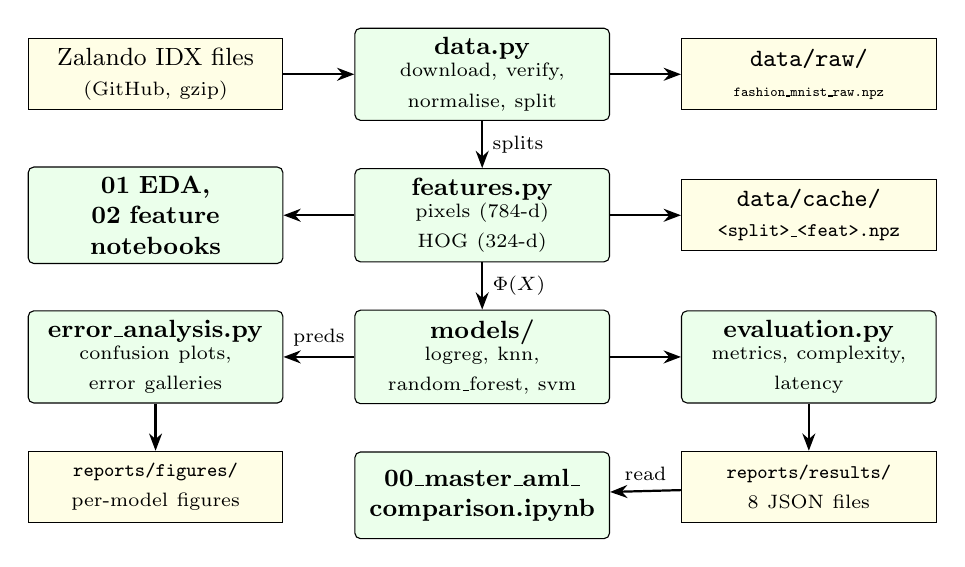
\begin{tikzpicture}[
    node distance=6mm and 9mm,
    box/.style={draw, rounded corners=2pt, align=center, minimum height=11mm,
                text width=30mm, font=\small, fill=green!8},
    store/.style={draw, align=center, font=\small, text width=30mm,
                  minimum height=9mm, fill=yellow!10},
    arr/.style={-{Stealth[length=2.2mm]}, thick},
  ]
  % Row 1: data acquisition
  \node[store] (zal) {Zalando IDX files\\\scriptsize (GitHub, gzip)};
  \node[box, right=of zal] (data) {\textbf{data.py}\\\scriptsize download, verify,\\normalise, split};
  \node[store, right=of data] (raw) {\file{data/raw/}\\\tiny \file{fashion\_mnist\_raw.npz}};

  % Row 2: features
  \node[box, below=of data] (feat) {\textbf{features.py}\\\scriptsize pixels (784-d)\\HOG (324-d)};
  \node[store, right=of feat] (cache) {\file{data/cache/}\\\scriptsize \file{<split>\_<feat>.npz}};
  \node[box, left=of feat] (nb1) {\textbf{01 EDA,}\\\textbf{02 feature notebooks}};

  % Row 3: models
  \node[box, below=of feat] (models) {\textbf{models/}\\\scriptsize logreg, knn,\\random\_forest, svm};
  \node[box, right=of models] (eval) {\textbf{evaluation.py}\\\scriptsize metrics, complexity,\\latency};
  \node[box, left=of models] (err) {\textbf{error\_analysis.py}\\\scriptsize confusion plots,\\error galleries};

  % Row 4: reporting
  \node[store, below=of eval] (json) {\scriptsize\file{reports/results/}\\8 JSON files};
  \node[box, below=of models] (master) {\textbf{00\_master\_aml\_}\\\textbf{comparison.ipynb}};
  \node[store, below=of err] (figs) {\scriptsize\file{reports/figures/}\\per-model figures};

  \draw[arr] (zal) -- (data);
  \draw[arr] (data) -- (raw);
  \draw[arr] (data) -- node[right, font=\scriptsize] {splits} (feat);
  \draw[arr] (feat) -- (cache);
  \draw[arr] (feat) -- (nb1);
  \draw[arr] (feat) -- node[right, font=\scriptsize] {$\Phi(X)$} (models);
  \draw[arr] (models) -- (eval);
  \draw[arr] (models) -- node[above, font=\scriptsize] {preds} (err);
  \draw[arr] (eval) -- (json);
  \draw[arr] (json) -- node[above, font=\scriptsize] {read} (master);
  \draw[arr] (err) -- (figs);
\end{tikzpicture}
\caption{End-to-end Phase~1 system architecture and pipeline data flow.
Green nodes represent executable package modules and analysis notebooks;
yellow nodes represent disk storage. Large raw datasets and feature caches
are excluded from version control via \file{.gitignore}; evaluation metrics
and generated PNG figures are committed.}
\label{fig:arch}
\end{figure*}

\subsection{Data Contracts}
To prevent implicit type conversions and silent shape corruptions, all
inter-module communication strictly conforms to the interface contracts
specified in Table~\ref{tab:contracts}.

\begin{table}[!t]
\centering
\caption{Strict Array Contracts Governing Inter-Module Communication}
\label{tab:contracts}
\footnotesize
\setlength{\tabcolsep}{4pt}
\begin{tabularx}{\columnwidth}{@{}lll>{\raggedright\arraybackslash}X@{}}
\toprule
Artefact & Shape & dtype & Value Domain \& Constraints\\
\midrule
Raw Images     & $(N, 28, 28)$ & \code{float32} & $[0.0, 1.0]$, finite, non-NaN\\
Ground Truth   & $(N,)$        & \code{int64}   & Categorical label $\in \{0,\dots,9\}$\\
Pixel Features & $(N, 784)$    & \code{float32} & $[0.0, 1.0]$, row-major flattened\\
HOG Features   & $(N, 324)$    & \code{float32} & $\ge 0.0$, block-normalised (L2-Hys)\\
\bottomrule
\end{tabularx}
\end{table}

\subsection{Standardized Experimental Protocol}
\label{sec:protocol}
To prevent data leakage, model selection and final evaluation are decoupled
via a strict three-way partitioning protocol (Fig.~\ref{fig:splits}).
The official $60{,}000$-sample training set is partitioned using stratified
shuffling (\code{StratifiedShuffleSplit}, seed $42$) into:
\begin{itemize}
  \item a \emph{training split} ($48{,}000$ images) used exclusively for
    fitting candidate hyperparameters across predefined grids;
  \item a \emph{validation split} ($12{,}000$ images, $20\%$ of training data)
    used strictly for model selection;
  \item a \emph{held-out test split} ($10{,}000$ images) provided by the
    official benchmark, which remains completely sealed until final model
    refitting.
\end{itemize}

\begin{figure*}[!t]
\centering
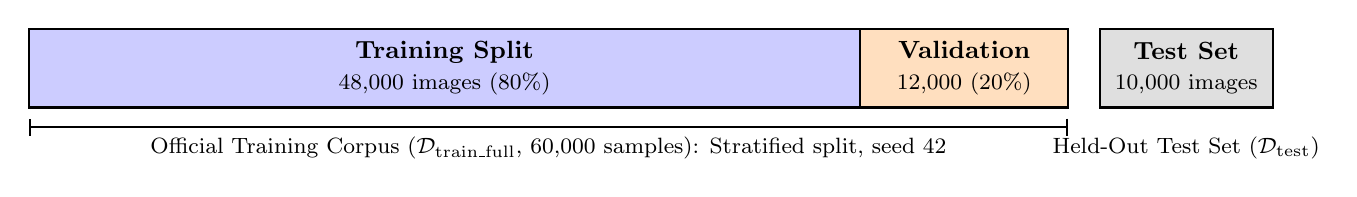
\begin{tikzpicture}[font=\small]
  \fill[blue!20]   (0,0)     rectangle (10.56,1.0);
  \fill[orange!25] (10.56,0) rectangle (13.20,1.0);
  \fill[gray!25]   (13.60,0) rectangle (15.80,1.0);
  \draw[thick] (0,0) rectangle (13.20,1.0);
  \draw[thick] (13.60,0) rectangle (15.80,1.0);
  \draw[thick] (10.56,0) -- (10.56,1.0);
  \node at (5.28,0.5) [align=center] {\textbf{Training Split}\\\footnotesize 48{,}000 images (80\%)};
  \node at (11.88,0.5) [align=center] {\textbf{Validation}\\\footnotesize 12{,}000 (20\%)};
  \node at (14.70,0.5) [align=center] {\textbf{Test Set}\\\footnotesize 10{,}000 images};
  \draw[|-|, thick] (0,-0.25) -- (13.20,-0.25);
  \node[below] at (6.60,-0.25)
       {\footnotesize Official Training Corpus ($\mathcal{D}_{\text{train\_full}}$, 60{,}000 samples): Stratified split, seed 42};
  \node[below] at (14.70,-0.25) {\footnotesize Held-Out Test Set ($\mathcal{D}_{\text{test}}$)};
\end{tikzpicture}
\caption{Three-way dataset partitioning scheme. Hyperparameter tuning is
performed strictly on the $48\text{k}/12\text{k}$ split. The winning
hyperparameter tuple is refitted on all $60{,}000$ training images prior to
a single evaluation on the $10{,}000$ test images.}
\label{fig:splits}
\end{figure*}

For each model and feature representation, candidate hyperparameter
combinations are evaluated on the validation split. The candidate
maximising macro-$F_1$ is selected (ties broken by first candidate index).
The winning configuration is subsequently refitted on all $60{,}000$
training images ($\mathcal{D}_{\text{train\_full}}$) and evaluated exactly
once on the test set ($\mathcal{D}_{\text{test}}$). Table~\ref{tab:grids}
outlines the explored hyperparameter search grids.

\begin{table*}[!t]
\centering
\caption{Classifier Implementations and Hyperparameter Tuning Grids}
\label{tab:grids}
\begin{tabularx}{\textwidth}{>{\raggedright\arraybackslash}p{2.6cm}
                             >{\raggedright\arraybackslash}X
                             >{\raggedright\arraybackslash}p{4.8cm}}
\toprule
Model Family & Pipeline Architecture \& Preprocessing & Validation Tuning Grid\\
\midrule
Logistic Regression & \code{StandardScaler} $\to$
  \code{LogisticRegression(solver="lbfgs", max\_iter=2000, random\_state=42)};
  Multinomial cross-entropy over 10 classes
  & Regularisation $C \in \{0.1, 1.0, 10.0\}$\\
\addlinespace[3pt]
$k$-Nearest Neighbours & \code{KNeighborsClassifier(algorithm="brute", metric="euclidean")};
  Chunked matrix prediction (\code{batch\_size=500})
  & Neighbours $k \in \{3, 5, 7, 9\}$;\newline
    Weighting $\in \{\text{uniform}, \text{distance}\}$\\
\addlinespace[3pt]
Random Forest & Multi-threaded \code{RandomForestClassifier(n\_jobs=-1, random\_state=42)};
  Unscaled features (scale-invariant splits)
  & Estimators $n_{\text{trees}} \in \{50, 100, 200\}$;\newline
    Max Depth $\in \{10, 20, \text{None}\}$\\
\addlinespace[3pt]
Linear SVM & \code{StandardScaler(with\_mean=False)} $\to$
  \code{LinearSVC(max\_iter=2000, dual="auto", random\_state=42)};
  One-vs-Rest (OvR) formulation
  & Regularisation $C \in \{0.1, 1.0, 10.0\}$\\
\bottomrule
\end{tabularx}
\end{table*}

\subsection{Result Serialization Schema and Master Synthesis}
Every model execution exports an immutable JSON record to
\file{reports/results/<model>\_<features>.json}. The schema enforces
strict typing: model identifiers, chosen parameters, split dimensions,
validation and test accuracy, validation and test macro-$F_1$, ten
per-class recall floats, parameter complexity counts, median inference
latencies, and the full $10\times 10$ integer test confusion matrix.

The synthesis notebook
(\repopath{00_master_aml_comparison.ipynb}) consumes
only these serialised records. To ensure absolute data integrity, the
master notebook performs schema assertion: it verifies non-empty fields,
finite bounds in $[0.0, 1.0]$, ten distinct class recalls, integer split
sizes, and non-negative complexity metrics. Synthesis tables and
comparative figures are rendered only after all eight records pass
validation.

% =====================================================================
\section{Implementation Details}
\label{sec:impl}

\subsection{Data Acquisition and Ingestion (\file{data.py})}
The dataset ingestion module downloads the four canonical Fashion-MNIST
gzip archives directly from Zalando's public repository. Data integrity is
enforced through a multi-stage validation sequence:
\begin{enumerate}
  \item \emph{Cryptographic Digest Verification:} The raw payload's MD5
    checksum is validated against the official published hash prior to
    decompression, preventing truncated or corrupted network downloads.
  \item \emph{Binary IDX Header Verification:} Unpacked bytes are parsed
    using big-endian binary struct unpacking. The magic header is
    validated against $\mathtt{0x0800} + r$, where $r=3$ for images and
    $r=1$ for label vectors, confirming shape dimensions $(N, 28, 28)$
    and $(N,)$ respectively.
  \item \emph{In-Place Normalisation:} Raw $\code{uint8}$ byte values
    $p \in \{0, \dots, 255\}$ are scaled to single-precision floating-point
    values $x = p / 255.0 \in [0.0, 1.0]$ directly in \code{float32} using
    NumPy, avoiding temporary \code{float64} memory allocation.
  \item \emph{Atomic Cache Serialisation:} The processed arrays are written
    to a temporary archive and renamed atomically via POSIX
    \code{Path.replace} to \repopath{data/raw/fashion_mnist_raw.npz}.
    Later invocations reload and validate the cache without network access.
\end{enumerate}

\subsection{Exploratory Data Analysis}
The ten categories are balanced: each contributes $4{,}800$ development
training images, $1{,}200$ validation images, and $1{,}000$ test images.
Differences in per-class recall therefore cannot
be attributed to unequal class counts. Exploratory analysis of class
means, variances, and a two-dimensional PCA projection indicates similar
upper-body silhouettes and overlapping garment distributions. The PCA
projection is descriptive rather than proof of inseparability in the
full feature space.

\subsection{Feature Engineering and Representations (\file{features.py})}

\subsubsection{Representation 1: Raw Flattened Pixels (784-d)}
The baseline representation reshapes each $28\times 28$ image into a
$784$-dimensional row vector via standard C-contiguous flattening:
$\phi_{\text{pix}}(x)_{28r + c} = x_{rc}$. This mapping preserves all
photometric intensity information with minimal transformation cost.
The transformation retains the original coordinates, but does not give
the downstream estimators an explicit local-neighbourhood structure or
translation invariance: shifting an object changes its vector coordinates.

\subsubsection{Representation 2: Histogram of Oriented Gradients (324-d)}
The HOG descriptor~\cite{dalal2005hog} models local shape by encoding the
spatial distribution of intensity gradients, implemented via
scikit-image. Given an image $x$, horizontal
and vertical gradients $g_u = \frac{\partial x}{\partial u}$ and
$g_v = \frac{\partial x}{\partial v}$ are computed via 1D centered point
derivative masks. Gradient magnitude and unsigned orientation are derived as:
\begin{align}
  m(u, v) &= \sqrt{g_u^2 + g_v^2},\\
  \theta(u, v) &= \operatorname{atan2}(g_v,g_u) \bmod 180^\circ.
\end{align}
The feature extraction parameters are configured as follows:
\begin{itemize}
  \item \emph{Cell Dimensions:} $7\times 7$ pixels per spatial cell,
    yielding $(28/7) = 4$ cells along each axis ($16$ total cells).
  \item \emph{Orientation Quantization:} 9 unsigned angular bins spanning
    $0^\circ$ to $180^\circ$ ($20^\circ$ per bin), weighted by gradient
    magnitude $m(u,v)$.
  \item \emph{Block Normalization:} $2\times 2$ cells per block with a
    stride of 1 cell ($3\times 3 = 9$ overlapping blocks).
  \item \emph{L2-Hys Contrast Normalisation:} Each 36-dimensional block
    vector $v$ undergoes standard L2 normalisation, value clipping at
    $\tau = 0.2$, and secondary L2 re-normalisation:
    \begin{align}
      v' &= \frac{v}{\sqrt{\|v\|_2^2 + \epsilon^2}}, \quad
      v'' = \min(v', 0.2),\\
      \hat{v} &= \frac{v''}{\sqrt{\|v''\|_2^2 + \epsilon^2}}.
    \end{align}
\end{itemize}
The resulting descriptor dimensionality is:
\begin{equation}
  d_{\text{HOG}} = \underbrace{(4 - 2 + 1)^2}_{\text{blocks}=9} \times
  \underbrace{(2 \times 2)}_{\text{cells/block}} \times
  \underbrace{9}_{\text{bins}} = 324.
\end{equation}
Compared to raw pixels, HOG achieves a $58.7\%$ dimensionality reduction
($784 \to 324$), providing local illumination invariance and slight spatial
shift tolerance.

\begin{figure}[!t]
\centering
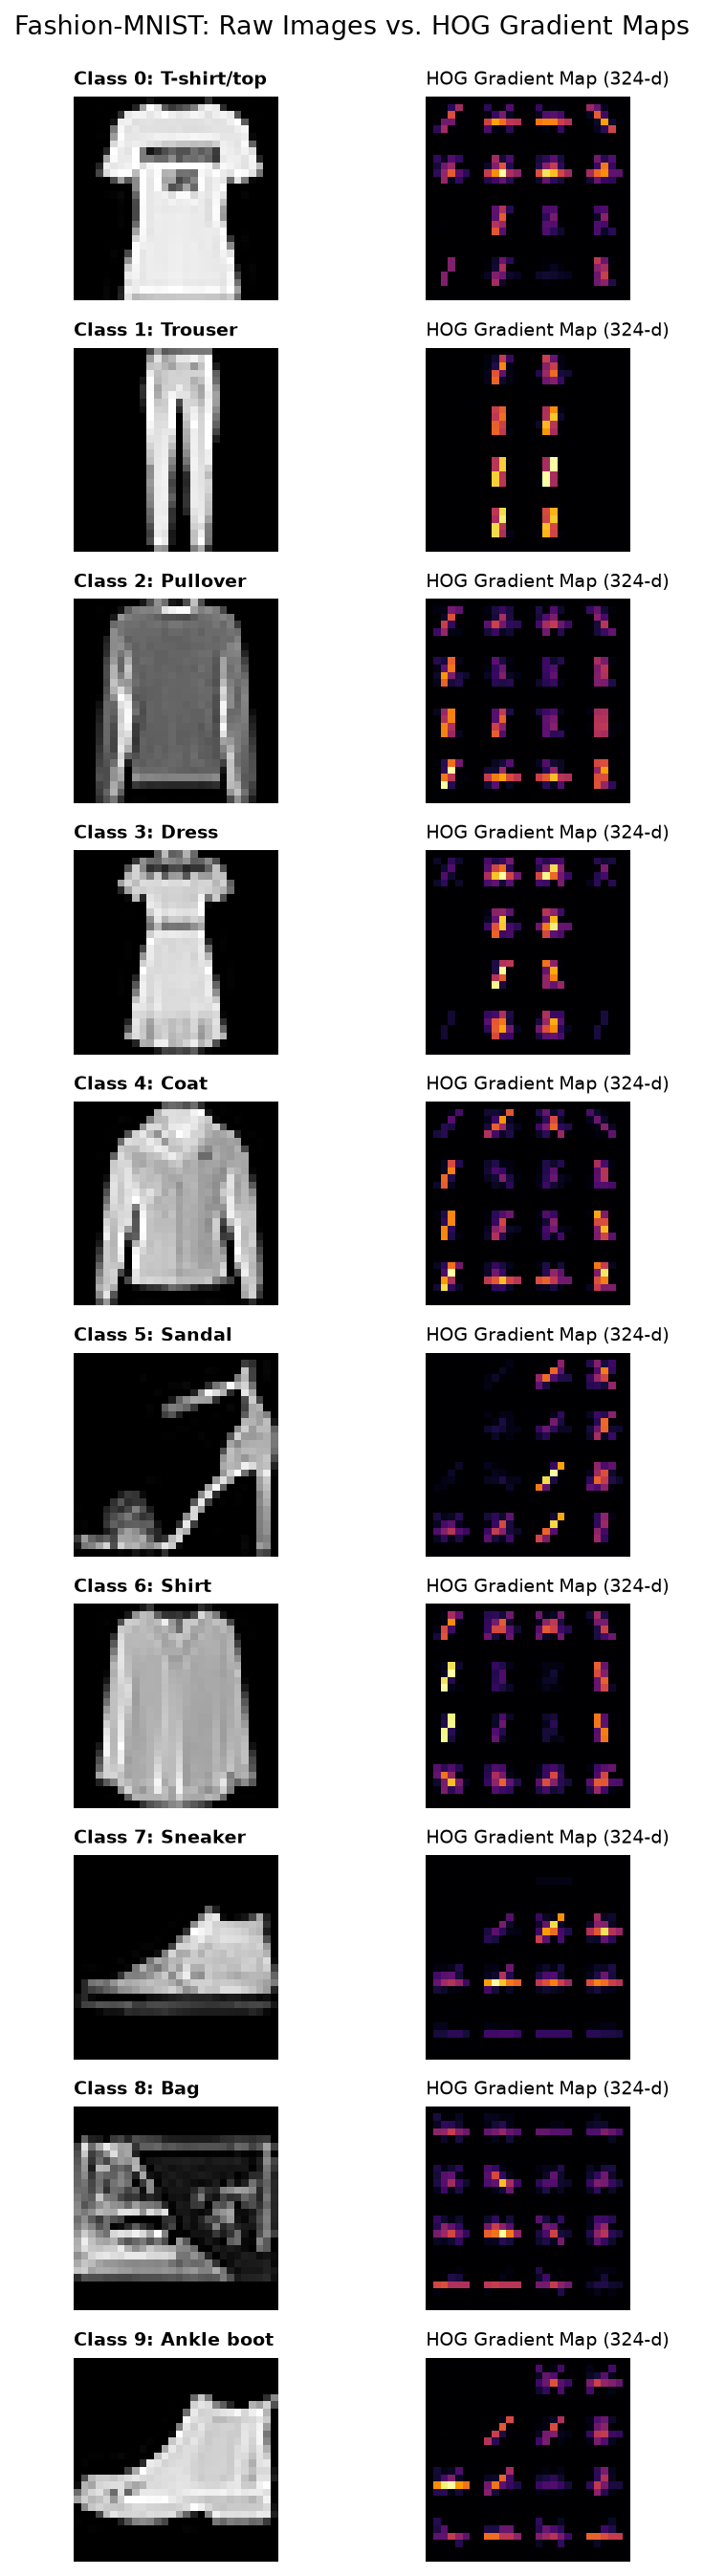
\includegraphics[height=0.55\textheight, width=\columnwidth,
                 keepaspectratio]{features/hog_vs_pixels.png}
\caption{Qualitative comparison of raw $28\times 28$ images (left) and their
corresponding HOG visualisations (right), with one training exemplar per
category. The visualisation shows pooled gradient structure rather than
a reconstruction of the original image.}
\label{fig:hog}
\end{figure}

Fig.~\ref{fig:hog} illustrates raw training samples alongside their
extracted HOG gradient vector fields. Garments with pronounced structural
silhouettes (e.g., Trouser, Sandal, Bag) produce highly distinctive
gradient fields. Conversely, upper-body garments (Pullover, Coat, Shirt)
display remarkably similar isotropic gradient fields. Crucial diagnostic
features---such as button plackets, neckbands, and collar lapels---may
occupy only a few pixels at $28\times 28$ resolution and
can be attenuated by the $7\times 7$ cell pooling operation.

\subsection{Standardized Evaluation Suite (\file{evaluation.py})}

\subsubsection{Classification Performance Metrics}
Classification quality is assessed using strict macro-averaged metrics
implemented in scikit-learn~\cite{pedregosa2011sklearn}:
\begin{align}
  \text{Accuracy} &= \frac{1}{n} \sum_{i=1}^{n} \mathbf{1}[\hat{y}_i = y_i],\\
  \text{Recall}_k &= \frac{\mathrm{TP}_k}{\mathrm{TP}_k + \mathrm{FN}_k}, \quad
  \text{Precision}_k = \frac{\mathrm{TP}_k}{\mathrm{TP}_k + \mathrm{FP}_k},\\
  \text{Macro-}F_1 &= \frac{1}{10} \sum_{k=0}^{9} \frac{2 \cdot \text{Precision}_k \cdot \text{Recall}_k}{\text{Precision}_k + \text{Recall}_k}.
\end{align}
Enforcing uniform $10\%$ class weighting in Macro-$F_1$ ensures that
failure on difficult categories cannot be masked by
flawless classification on easier categories.

\subsubsection{Model Complexity and Storage Quantification}
Parameter complexity is recorded according to model structure:
\begin{itemize}
  \item for linear models (Logistic Regression, Linear SVM), complexity
    equals total learnable weights plus intercepts: $10d + 10$ ($7{,}850$
    for pixels, $3{,}250$ for HOG);
  \item for Random Forests, complexity is measured as the total number of
    decision nodes summed across all constituent trees;
  \item for non-parametric $k$-NN, which retains training data rather than
    learning weights, complexity is quantified by active memory footprint:
    $M = (N \cdot d \cdot 4) / 2^{20}$~MiB ($179.4$~MiB for pixels,
    $74.2$~MiB for HOG across $60{,}000$ \code{float32} vectors).
\end{itemize}

\subsubsection{Empirical Inference Latency Benchmarking}
Latency is measured on a dedicated batch of $B = 1{,}000$ test samples
following a ten-sample pipeline warm-up. Timing is captured over $T = 5$
independent iterations using \code{time.perf\_counter}:
\begin{equation}
  \text{Latency} = 10^3 \cdot \operatorname*{median}_{t=1,\dots,T}
  \left(\frac{\Delta t}{B}\right) \quad (\text{ms per image}).
\end{equation}
Reporting the median mitigates transient operating system scheduling jitter.
Feature extraction is excluded; these are amortised batch prediction
times rather than end-to-end single-image response times.

\subsection{Classifier Model Architectures (\file{models/})}
All four classifier modules expose a consistent tuning and evaluation
interface. Logistic Regression and Linear SVM use scikit-learn
\code{Pipeline} objects for scaling; $k$-NN and Random Forest use
estimators directly:
\begin{itemize}
  \item \emph{Logistic Regression:} Configured with \code{StandardScaler}
    and multinomial cross-entropy optimised via the quasi-Newton L-BFGS
    algorithm. A $2{,}000$-iteration limit allows longer optimisation runs;
    convergence should still be checked for each fit.
  \item \emph{$k$-Nearest Neighbours:} Uses brute-force Euclidean distance
    computation. Predictions are batched in chunks of $500$ queries to
    constrain peak memory allocation.
  \item \emph{Random Forest:} Multi-threaded ensemble (\code{n\_jobs=-1})
    utilising Gini impurity splits. Features remain unscaled, preserving
    natural intensity thresholds.
  \item \emph{Linear SVM:} Implemented via \code{LinearSVC} with squared-hinge
    loss in a One-vs-Rest configuration. Features are scaled without
    centring (\code{with\_mean=False}) to preserve sparsity.
\end{itemize}

\subsection{Verification and Unit Testing Suite}
To guarantee software reliability, the \file{tests/} directory houses 35
unit tests spanning six modules executed via Python's \code{unittest}
framework. Tests run entirely offline without network access using
synthetic broadcasted arrays. Test coverage encompasses:
\begin{itemize}
  \item data integrity, checksum verification, and stratified split
    reproducibility (\file{test\_foundation.py}, 9 tests);
  \item feature extraction shapes, dtypes, and cache serialization
    (\file{test\_features.py}, 7 tests);
  \item pipeline construction, hyperparameter grid search, and schema
    validation for all four classifier modules (\file{test\_logreg.py},
    \file{test\_knn.py}, \file{test\_svm.py}, 16 tests);
  \item master notebook schema validation and report parsing
    (\file{test\_master\_notebook.py}, 3 tests).
\end{itemize}
The suite verifies the shared contracts and export schema independently
of the full training runs.

% =====================================================================
\section{Experimental Results and Discussion}
\label{sec:results}

All empirical metrics reported herein are extracted directly from the eight
audited JSON records serialised on the held-out $10{,}000$-image test set.

\subsection{Master Benchmark Evaluation}
Table~\ref{tab:results} presents the comparative evaluation across all
eight Phase~1 configurations.

\begin{table*}[!t]
\centering
\caption{Phase~1 Master Applied Machine Learning Benchmark Results on
Fashion-MNIST Held-Out Test Set. Latency Measured as Median Milliseconds
per Image across 1{,}000 Queries. Best Test Scores in Bold}
\label{tab:results}
\footnotesize
\setlength{\tabcolsep}{4pt}
\begin{tabular}{lllrrrrr}
\toprule
Model Family & Feature Space & Optimal Parameters & Val.\ Acc.\ (\%) & Test Acc.\ (\%) & Test Macro-$F_1$ (\%) & Latency (ms) & Model Complexity\\
\midrule
Log.\ Regression & Pixels (784-d) & $C=0.1$ & 85.97 & 84.32 & 84.24 & 0.00073 & 7,850 weights\\
Log.\ Regression & HOG (324-d)    & $C=0.1$ & 85.51 & 84.55 & 84.49 & 0.00037 & 3,250 weights\\
$k$-NN           & Pixels (784-d) & $k=7$, distance & 86.03 & 85.41 & 85.40 & 0.27412 & 179.44 MiB (RAM)\\
$k$-NN           & HOG (324-d)    & $k=5$, distance & 84.75 & 83.84 & 83.85 & 0.09799 & 74.16 MiB (RAM)\\
Random Forest    & Pixels (784-d) & 200 trees, depth 20 & 88.57 & \textbf{87.43} & \textbf{87.31} & 0.02636 & 1,693,570 nodes\\
Random Forest    & HOG (324-d)    & 200 trees, depth None & 84.98 & 84.35 & 84.30 & 0.02913 & 2,458,016 nodes\\
Linear SVM       & Pixels (784-d) & $C=0.1$ & 85.72 & 83.80 & 83.57 & 0.00133 & 7,850 weights\\
Linear SVM       & HOG (324-d)    & $C=1.0$ & 85.31 & 84.23 & 84.06 & 0.00060 & 3,250 weights\\
\bottomrule
\end{tabular}
\end{table*}

The benchmark demonstrates that the Random Forest on raw pixels achieves
the highest overall test accuracy and macro-$F_1$:
$87.43\%$ test accuracy and $87.31\%$ macro-$F_1$. The remaining seven
configurations plateau within a narrow performance envelope between
$83.80\%$ and $85.41\%$. Notably, expanding model complexity from
$3{,}250$ parameters (Linear SVM) to nearly $2.5$ million nodes (Random
Forest on HOG) produces less than a $0.55\%$ accuracy improvement,
suggesting diminishing returns within the evaluated model families and
feature representations.

\subsection{Impact of Feature Representation: Pixels vs. HOG}
Evaluating classifiers across both feature spaces reveals a distinct
divergence between linear and non-linear models:
\begin{itemize}
  \item \emph{Linear Classifiers Benefit from HOG:} Multinomial Logistic
    Regression gains $+0.23$ percentage points ($84.32\% \to 84.55\%$),
    while Linear SVM gains $+0.43$ points ($83.80\% \to 84.23\%$). HOG's
    gradient binning effectively linearises local edge structures, enabling
    hyperplanes to separate global silhouettes more cleanly.
  \item \emph{Non-Linear Classifiers Degrade with HOG:} $k$-NN accuracy
    drops by $-1.57$ points ($85.41\% \to 83.84\%$), and Random Forest
    accuracy drops substantially by $-3.08$ points ($87.43\% \to 84.35\%$).
    Because decision trees split along orthogonal coordinate axes, raw
    pixel intensities provide sharp, unpooled threshold boundaries. HOG's
    $7\times 7$ cell averaging blurs these discrete pixel intensities,
    depriving trees of high-frequency spatial cues.
\end{itemize}

\subsection{Overfitting Dynamics and Model Interpretability}
Fig.~\ref{fig:rf} illustrates the validation trajectory of the Random
Forest across tree depth. When depth is unconstrained (\code{max\_depth=None}),
the forest memorises $100\%$ of the training set across all tree counts,
while validation accuracy plateaus at $88.38\%$ for pixels and $84.98\%$
for HOG with 200 trees. The selected pixel model uses depth 20; the
selected HOG model uses unrestricted depth. Their refitted node counts
in Table~\ref{tab:results} describe different feature spaces and should
not be interpreted as the effect of depth alone.

\begin{figure*}[!t]
\centering
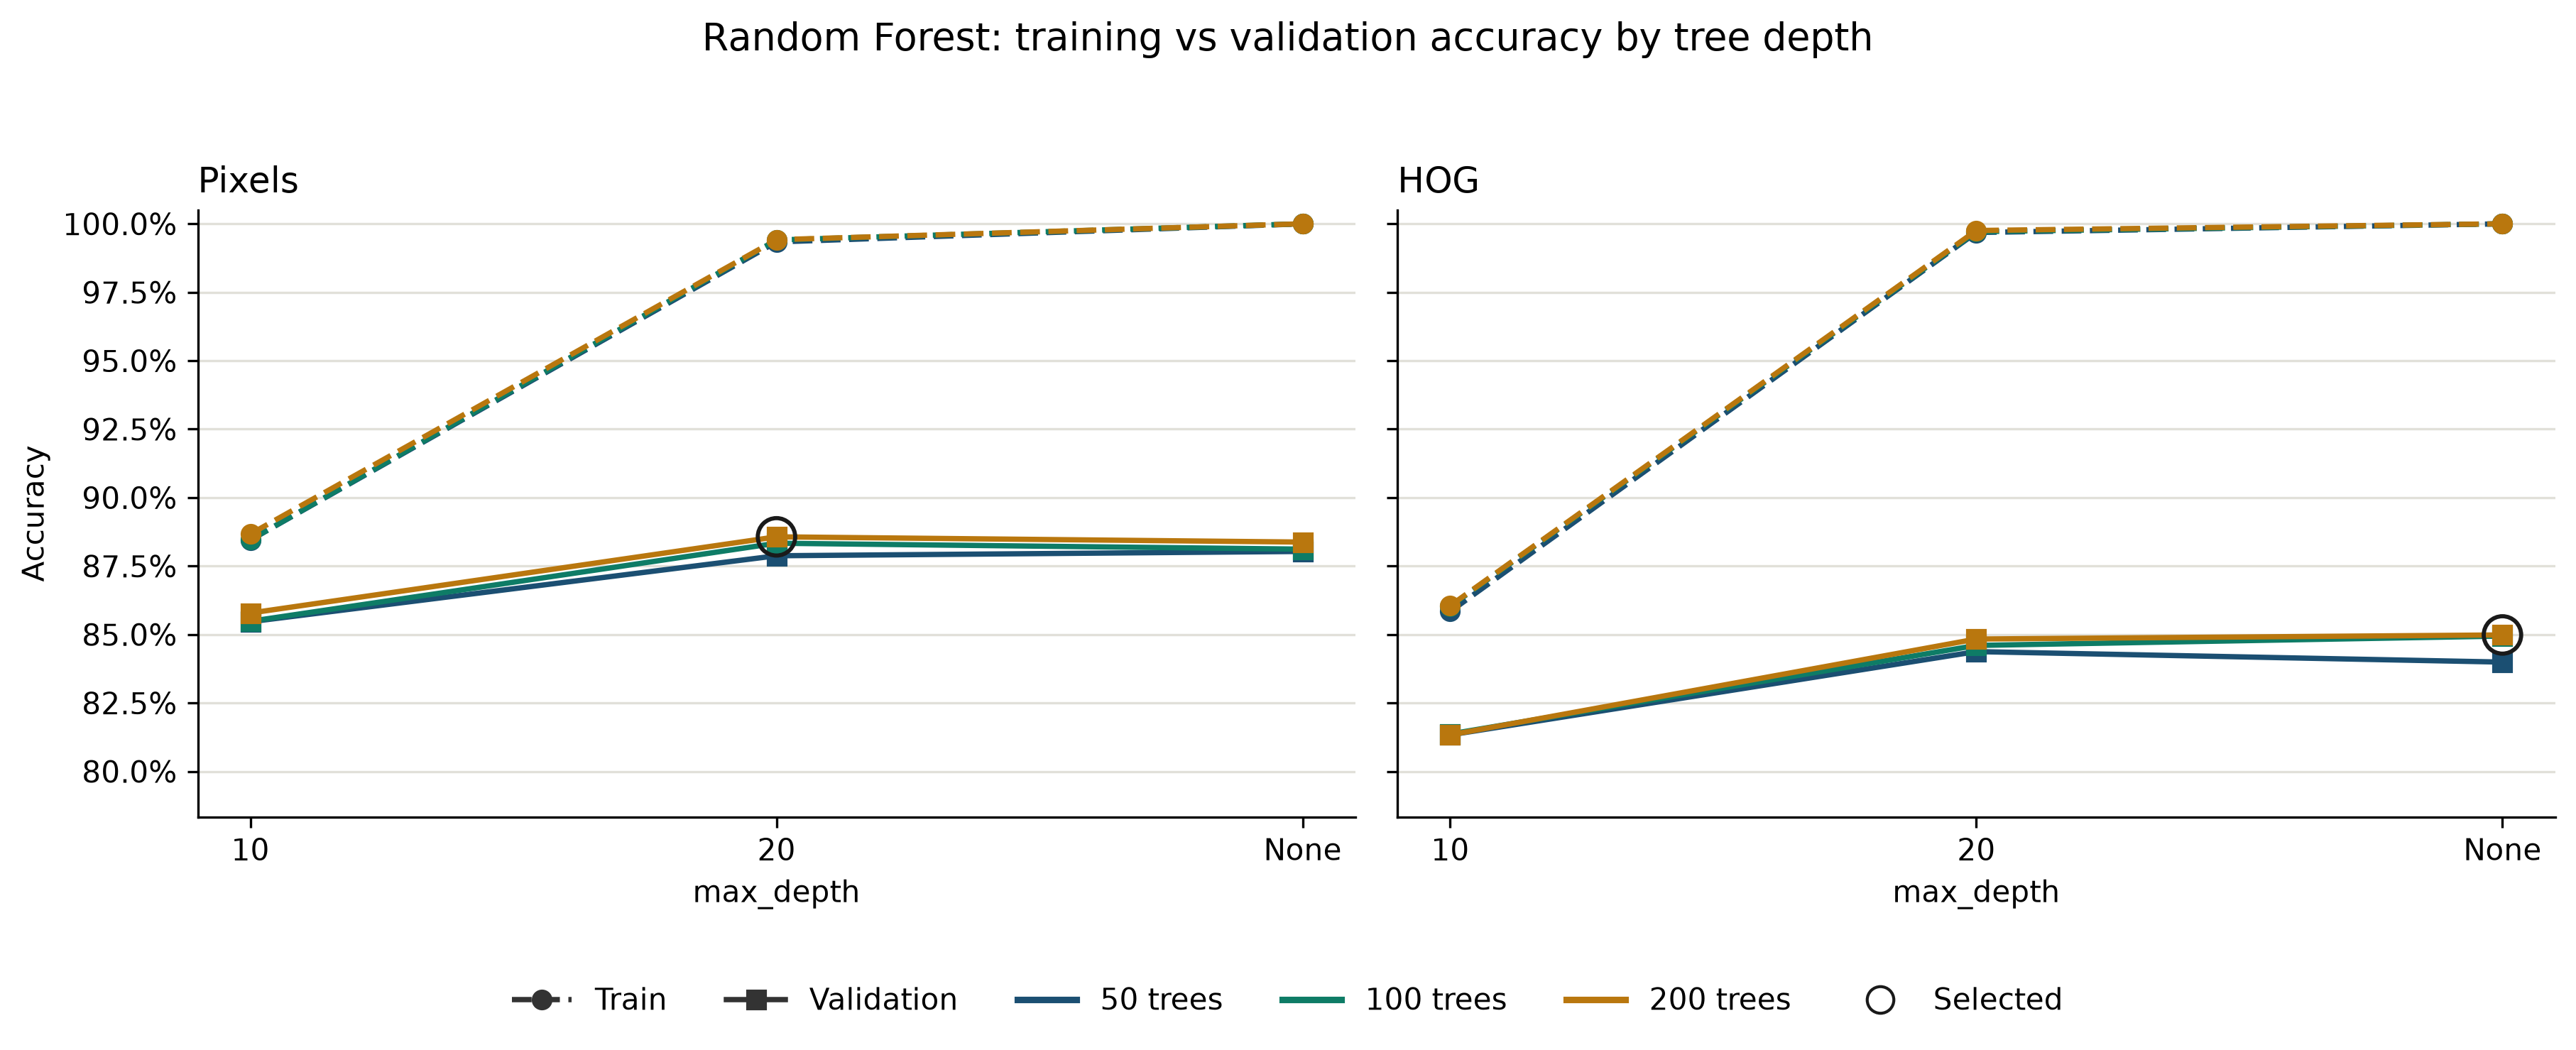
\includegraphics[width=0.88\textwidth]{rf/overfitting_curves.png}
\caption{Random Forest training and validation accuracy across maximum
tree depth, shown separately for pixels and HOG. Unrestricted depth fits
the training data almost perfectly while validation accuracy plateaus.
The selected pixel configuration uses 200 trees and depth 20.}
\label{fig:rf}
\end{figure*}

Fig.~\ref{fig:logreg} provides spatial interpretability by reshaping the
$784$ learned logistic regression weights back into $28\times 28$ image
grids. Positive coefficients (red) trace the distinctive structural
outlines of specific categories (e.g., trouser leg contours, bag handles),
while negative coefficients (blue) actively suppress confounding spatial
regions (e.g., collar zones for crewneck tops).

\begin{figure*}[!t]
\centering
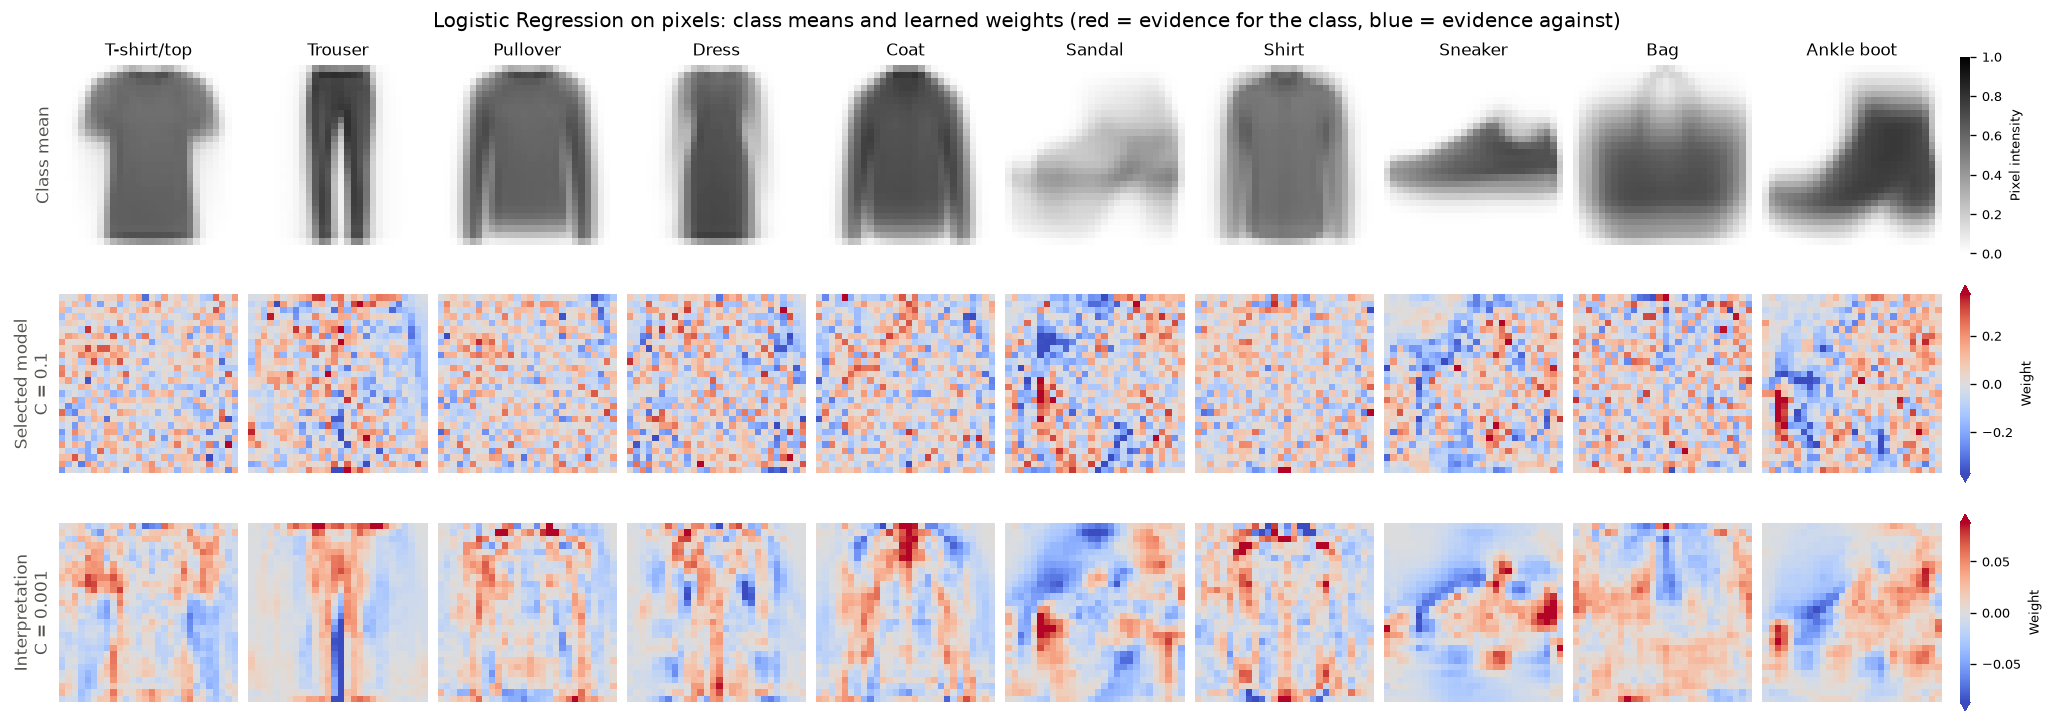
\includegraphics[width=\textwidth]{logreg/pixel_weight_heatmaps.png}
\caption{Spatial weight heatmaps for Multinomial Logistic Regression reshaped
into $28\times 28$ grids. Top: empirical class means; Middle: learned weights
under optimal regularisation ($C=0.1$); Bottom: weights under heavy
regularisation ($C=0.001$) isolating class silhouette templates. Red
indicates positive class evidence; blue indicates inhibitory suppression.}
\label{fig:logreg}
\end{figure*}

Random Forest Gini importance provides a complementary view of
coordinate usage, with important pixels inside the garment region as
well as around boundaries. It summarises split usage rather than
providing a causal or class-specific explanation.

\subsection{Per-Class Recall and ``The Gap''}
Table~\ref{tab:recall} itemises test recall across all ten categories. A
pronounced dichotomy emerges between structured and unstructured apparel:
\begin{itemize}
  \item \emph{Structured Categories:} Trouser and Bag achieve
    $92.6\%$--$97.3\%$ recall across configurations. Footwear is usually
    well separated, although Sandal recall falls to $80.4\%$ for pixel
    $k$-NN, so this pattern does not apply uniformly to all footwear.
  \item \emph{The Shirt Failure Mode:} Shirt (Class 6) recall collapses
    drastically to $50.7$--$62.6\%$ across all eight models. This represents
    a deficit of $33.1$--$44.7$ percentage points relative to Trouser
    within the same configuration.
\end{itemize}

\begin{table*}[!t]
\centering
\caption{Per-Class Test Set Recall (\%). Shirt (Class 6) Exhibits a Catastrophic Deficit across All Models (Bold)}
\label{tab:recall}
\setlength{\tabcolsep}{4.5pt}
\begin{tabular}{llrrrrrrrrrr}
\toprule
Model & Features & T-shirt & Trouser & Pullover & Dress & Coat & Sandal & Shirt & Sneaker & Bag & Ankle boot\\
\midrule
Log.\ Reg. & Pixels & 80.6 & 95.8 & 73.7 & 86.1 & 76.0 & 92.1 & \textbf{57.1} & 93.8 & 93.2 & 94.8\\
Log.\ Reg. & HOG    & 80.6 & 94.8 & 73.0 & 85.2 & 75.5 & 93.3 & \textbf{57.8} & 92.7 & 97.2 & 95.4\\
$k$-NN     & Pixels & 84.8 & 96.7 & 80.3 & 86.7 & 77.0 & 80.4 & \textbf{60.2} & 95.6 & 95.3 & 97.1\\
$k$-NN     & HOG    & 80.2 & 95.7 & 71.7 & 79.6 & 74.0 & 87.5 & \textbf{62.6} & 95.3 & 96.6 & 95.2\\
Rand.\ Forest & Pixels & 85.9 & 96.1 & 78.9 & 90.5 & 81.1 & 95.6 & \textbf{59.3} & 95.2 & 97.3 & 94.4\\
Rand.\ Forest & HOG    & 81.2 & 92.6 & 73.6 & 85.5 & 74.7 & 94.0 & \textbf{59.4} & 90.8 & 96.9 & 94.8\\
Linear SVM & Pixels & 81.9 & 95.4 & 72.8 & 86.4 & 77.7 & 91.6 & \textbf{50.7} & 93.4 & 94.0 & 94.1\\
Linear SVM & HOG    & 80.0 & 94.8 & 73.4 & 86.4 & 73.8 & 93.1 & \textbf{54.6} & 93.9 & 97.1 & 95.2\\
\bottomrule
\end{tabular}
\end{table*}

\subsection{Quantified Upper-Body Confusion Analysis}
Table~\ref{tab:confusion} isolates the directional confusion pathways
responsible for the Shirt collapse. Across all configurations,
$32.3\%$ to $41.0\%$ of all test shirts are misclassified specifically as
other upper-body garments (T-shirt/top, Pullover, or Coat):
\begin{itemize}
  \item \emph{Shirt $\to$ T-shirt/top ($13.1$--$16.6\%$):} Short-sleeved
    and polo shirts lack prominent collar elevation at $28\times 28$
    resolution, causing classifiers to map them directly to crewnecks.
  \item \emph{Shirt $\to$ Pullover ($8.2$--$14.2\%$):} Long-sleeved
    dress shirts share torso volume, arm drape, and sleeve cuffs with
    sweaters.
  \item \emph{Shirt $\to$ Coat ($7.5$--$11.4\%$):} Heavy-weave buttoned
    shirts and dark plackets mimic outerwear lapels.
  \item \emph{Pullover $\to$ Coat ($8.4$--$16.8\%$):} Open cardigans
    frequently mimic the open front silhouette of coats.
\end{itemize}
Fig.~\ref{fig:upper} shows the upper-body sub-matrix for Linear SVM
on pixels. Percentages use each true class's full row count as the
denominator; the cropped sub-matrix is not renormalised.

\begin{table}[!t]
\centering
\caption{Directional Confusion Distribution for True Shirt Instances (\% of All 1{,}000 Test Shirts)}
\label{tab:confusion}
\resizebox{\columnwidth}{!}{%
\begin{tabular}{llrrrrrr}
\toprule
& & \multicolumn{5}{c}{True Shirt Classified As} & Pullover\\
\cmidrule(lr){3-7}
Model & Feat. & Shirt & T-shirt & Pullover & Coat & Upper-Body Sum & $\to$ Coat\\
\midrule
Log.\ Reg. & Pixels & 57.1 & 13.8 & 12.0 & 10.4 & 36.2 & 12.5\\
Log.\ Reg. & HOG    & 57.8 & 15.1 & 10.0 & 11.4 & 36.5 & 13.4\\
$k$-NN     & Pixels & 60.2 & 16.6 & 12.2 &  7.5 & 36.3 &  8.4\\
$k$-NN     & HOG    & 62.6 & 13.1 &  8.2 & 11.0 & 32.3 & 16.8\\
Rand.\ For.& Pixels & 59.3 & 14.8 & 12.0 &  9.0 & 35.8 & 13.0\\
Rand.\ For.& HOG    & 59.4 & 14.9 &  8.8 & 10.2 & 33.9 & 13.9\\
Linear SVM & Pixels & 50.7 & 15.6 & 14.2 & 11.2 & 41.0 & 14.0\\
Linear SVM & HOG    & 54.6 & 16.5 & 10.8 & 10.6 & 37.9 & 14.2\\
\bottomrule
\end{tabular}%
}
\end{table}

\begin{figure}[!t]
\centering
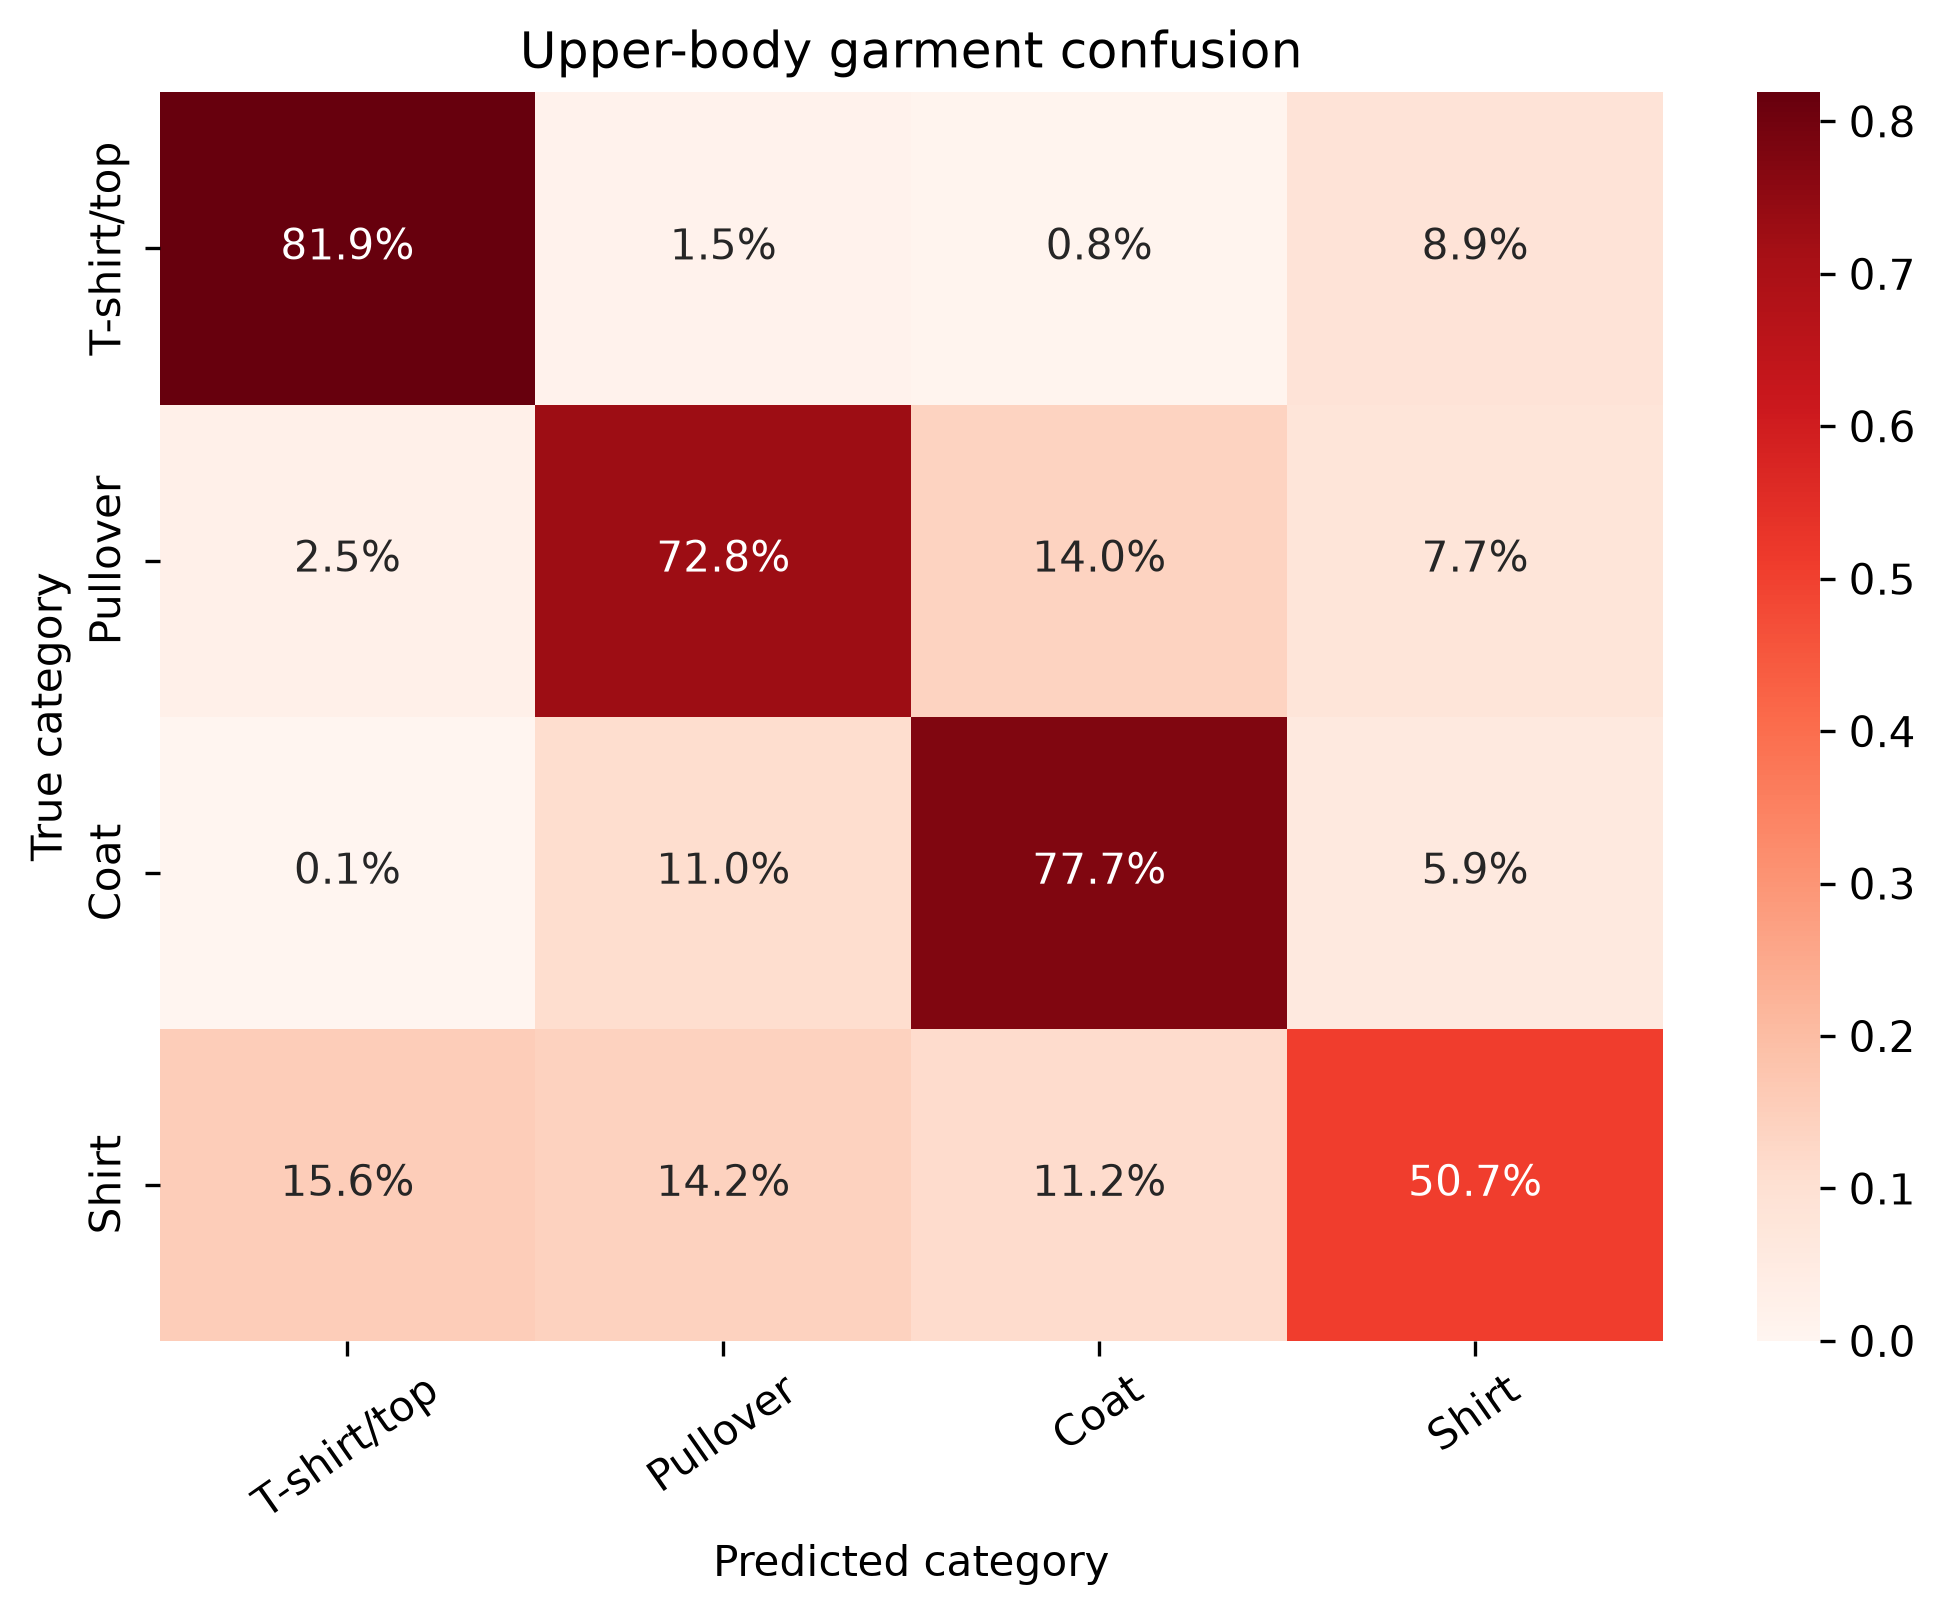
\includegraphics[width=\columnwidth]{errors/svm_pixels_upper_body_confusion.png}
\caption{Upper-body confusion for Linear SVM on raw pixels. Percentages
use all $1{,}000$ test examples of each true category as the denominator.
The Shirt row assigns $41.0\%$ to T-shirt/top, Pullover, and Coat combined.}
\label{fig:upper}
\end{figure}

These findings establish a shared weakness in the evaluated baselines.
They motivate testing learned spatial representations, but do not prove
an upper bound for every handcrafted descriptor or classical classifier.

\subsection{Qualitative Misclassification Examples}
Inspection of held-out images misclassified by the pixel Linear SVM
shows that Shirts predicted as T-shirt/top share short-sleeved
torso outlines; pullovers predicted as coats share long-sleeved silhouettes.
At $28\times 28$ resolution, fine neckline and front-opening details can
be difficult to distinguish. These examples support the ambiguity seen
in the confusion matrices, without identifying a definitive cause for
every prediction.

\subsection{Latency and Computational Scaling}
As reported in Table~\ref{tab:results}, inference latency spans three
orders of magnitude:
\begin{itemize}
  \item \emph{Linear Models ($0.00037$--$0.00133$~ms/image):} Linear SVM
    and Logistic Regression evaluate via a single dot-product matrix
    multiply ($W \cdot x + b$), making them highly suitable for
    high-throughput streaming catalogs.
  \item \emph{Random Forest ($0.02636$--$0.02913$~ms/image):} Tree
    traversals require parallel evaluation across 200 estimators.
  \item \emph{$k$-NN Bottleneck ($0.09799$--$0.27412$~ms/image):} $k$-NN
    scans $60{,}000$ stored vectors per query, creating a larger compute
    and storage requirement than the linear models.
\end{itemize}
At the benchmark batch size, HOG reduces recorded $k$-NN time by $64.2\%$
and stored feature memory by $58.7\%$. Timings from different developer
machines are indicative; controlled cross-model speed comparisons require
a shared host and runtime configuration.

% =====================================================================
\section{Conclusion and Phase 2 Roadmap}
\label{sec:conclusion}

\subsection{Summary of Phase 1 Findings}
Phase~1 successfully constructed an audited, reproducible applied machine
learning baseline for Fashion-MNIST clothing categorization:
\begin{enumerate}
  \item Classical classifiers achieve $83.80\%$ to $87.43\%$ test accuracy,
    led by Random Forest on raw pixels ($87.31\%$ macro-$F_1$).
  \item HOG feature extraction yields modest gains for linear models with
    $58.7\%$ fewer dimensions, but impairs tree and instance-based models.
  \item A catastrophic performance chasm exists between structured
    categories such as Trouser and Bag ($92.6$--$97.3\%$ recall) and
    Shirts ($50.7$--$62.6\%$ recall), with
    up to $41.0\%$ of shirts misclassified into adjacent tops.
\end{enumerate}

\subsection{Identified Limitations}
Several experimental limitations should be noted:
\begin{itemize}
  \item \emph{Single Random Seed:} Hyperparameter tuning utilised a single
    stratified split (seed 42); multi-seed cross-validation would provide
    tighter confidence intervals.
  \item \emph{Host Machine Heterogeneity:} Latency benchmarks reflect
    differing developer hardware configurations.
  \item \emph{Batch HOG Execution:} Feature extraction executed
    sequentially in Python rather than via multi-threaded C extensions.
\end{itemize}

\subsection{Phase 2 CNN Quantitative Targets}
Phase~1 establishes the exact empirical baseline that the Phase~2 small
Convolutional Neural Network must outperform. Phase~2 will evaluate a
compact CNN architecture on the exact same $10{,}000$-image test split
under identical evaluation standards. The quantitative success criteria
are defined as:
\begin{itemize}
  \item \textbf{Target 1 (Shirt Recall):} Elevate Shirt recall from the
    Phase~1 baseline of $50.7\%$--$62.6\%$ to $\mathbf{\ge 80.0\%}$.
  \item \textbf{Target 2 (Upper-Body Confusion):} Reduce misclassification
    of Shirts into T-shirts, Pullovers, and Coats from $32.3\%$--$41.0\%$
    down below $\mathbf{15.0\%}$.
  \item \textbf{Target 3 (Overall Generalization):} Improve test Macro-$F_1$
    beyond the best Phase~1 value of $87.31\%$ to $\mathbf{\ge 91.0\%}$.
\end{itemize}
These values are prospective targets; Phase~1 contains no trained CNN
or measured CNN results.

% =====================================================================
% Keep only directly cited background and implementation references.
\begin{thebibliography}{9}

\bibitem{xiao2017fashion}
H.~Xiao et al., ``Fashion-MNIST: A novel image dataset for benchmarking machine learning algorithms,'' arXiv:1708.07747, 2017.

\bibitem{liu2016deepfashion}
Z.~Liu et al., ``DeepFashion: Powering robust clothes recognition and retrieval with rich annotations,'' CVPR, 2016.

\bibitem{lecun1998mnist}
Y.~LeCun et al., ``Gradient-based learning applied to document recognition,'' \emph{Proc. IEEE}, 1998.

\bibitem{dalal2005hog}
N.~Dalal and B.~Triggs, ``Histograms of oriented gradients for human detection,'' CVPR, 2005.

\bibitem{cover1967knn}
T.~Cover and P.~Hart, ``Nearest neighbor pattern classification,'' \emph{IEEE Trans. Inf. Theory}, 1967.

\bibitem{breiman2001rf}
L.~Breiman, ``Random forests,'' \emph{Mach. Learn.}, 2001.

\bibitem{cortes1995svm}
C.~Cortes and V.~Vapnik, ``Support-vector networks,'' \emph{Mach. Learn.}, 1995.

\bibitem{krizhevsky2012imagenet}
A.~Krizhevsky et al., ``ImageNet classification with deep convolutional neural networks,'' NeurIPS, 2012.

\bibitem{pedregosa2011sklearn}
F.~Pedregosa et al., ``Scikit-learn: Machine learning in Python,'' \emph{JMLR}, 2011.

\end{thebibliography}

\end{document}
